\documentclass{article}
\usepackage[utf8]{inputenc}
\usepackage{hyperref}
\usepackage[letterpaper, portrait, margin=1in]{geometry}
\usepackage{enumitem}
\usepackage{amsmath}
\usepackage{amsthm}
\usepackage{booktabs}
\usepackage{graphicx}
\usepackage{float}
\usepackage{hyperref}
\usepackage[flushleft]{threeparttable}
\usepackage{textcomp}
\usepackage{amssymb}
\usepackage{dsfont}
\hypersetup{
colorlinks=true,
    linkcolor=black,
    filecolor=black,      
    urlcolor=blue,
    citecolor=black,
}
\usepackage{natbib}
\usepackage{yhmath}

\usepackage{titlesec}
\bibliographystyle{chicago}
\newcommand{\bib}{references.bib}
\newcommand\iid{\stackrel{\mathclap{iid}}{\sim}}
\newcommand\asym{\stackrel{\mathclap{a}}{\sim}}
\newcommand\convprob{\xrightarrow{p}}
\newcommand\convdist{\xrightarrow{d}}
\newcommand{\N}{\mathbb{N}}
\newcommand{\Z}{\mathbb{Z}}
\newcommand{\E}{\text{E}}
\newcommand{\V}{\text{Var}}
\newcommand{\Av}{\text{Avar}}
\newcommand{\se}{\text{se}}
\newcommand{\corr}{\text{Corr}}
\newcommand{\cov}{\text{Cov}}
\newcommand{\norm}{\text{Normal}}
\newcommand{\indep}{\perp \!\!\! \perp}

\begin{document}
% The tex content below is similar to the given main.tex
 
\title{Homework 5}
\author{Environmental Economics II\\
Maghfira Ramadhani}
\date{\today}
\maketitle

\section*{Problem 1 Python}
\begin{enumerate}
\item The OLS estimates from regression of price on $mpg$ with $car$ and a constant is -131.04. It means that more efficient car (higher $mpg$) is associated with lower price which does not make sense.
\item When estimateng the effect of fuel efficiency on price of vehicle, we should be careful with the endogeneity problem. The fuel efficiency of a vehicle is likely to be correlated with unobserved characteristics of the vehicle that are also correlated with the price of the vehicle. For example, the fuel efficiency of a vehicle may be correlated with the size of the vehicle, which is also correlated with the price of the vehicle. This is a problem because the OLS estimates will be biased and inconsistent.
\begin{enumerate}
    \item[(a)-(c)] Table \ref{t1:2SLS} show the by hand 2SLS estimates
    \begin{table}[H]\centering
    \caption{Two-stage least squares estimates of the effect of treatment on bycatch yield.}
    \label{t1:2SLS}
    \begin{threeparttable}
    \begin{tabular}{lccc}
\toprule
 & (a) & (b) & (c) \\
\midrule
Miles per gallon & 150.43 & 157.06 & 10165.74 \\
  & (59.30) & (57.56) & (25552.22) \\
=1 if the vehicle is sedan & -4676.09 & -4732.67 & -90156.39 \\
  & (548.94) & (537.90) & (218080.47) \\
\midrule Instrumental variable & Weight & Weight$^2$ & Height \\
First Stage F-statistic & 256.80 & 257.02 & 203.66 \\
\bottomrule
\end{tabular}

    \end{threeparttable}
    \end{table}
    
    \item[(d)] The instrumental variable must satisfy the relevancy conditions and exclusion restrictions. The relevancy condition requires that the instrument is correlated with the endogenous variable. The exclusion restriction requires that the instrument is not correlated with the error term, or in other words, the instrumental variable affect the outcome variable only through the endogenous variable. 
    
    Results from using the height of vehicle as the instrumental variable do not seems reasonable. I suspect that the exclusion restriction is not satisfied. The height of vehicle is likely to be correlated with whether or not the vehicle is sedan or SUV. Figure \ref{f1:exclusion} indicates that the height of vehicle is also affecting the price of vehicle through the type of vehicle, which violates the exclusion restriction.

    \begin{figure}[H]
    \centering
    % Input the figure from the figure file and order side by side and one in the bottom
    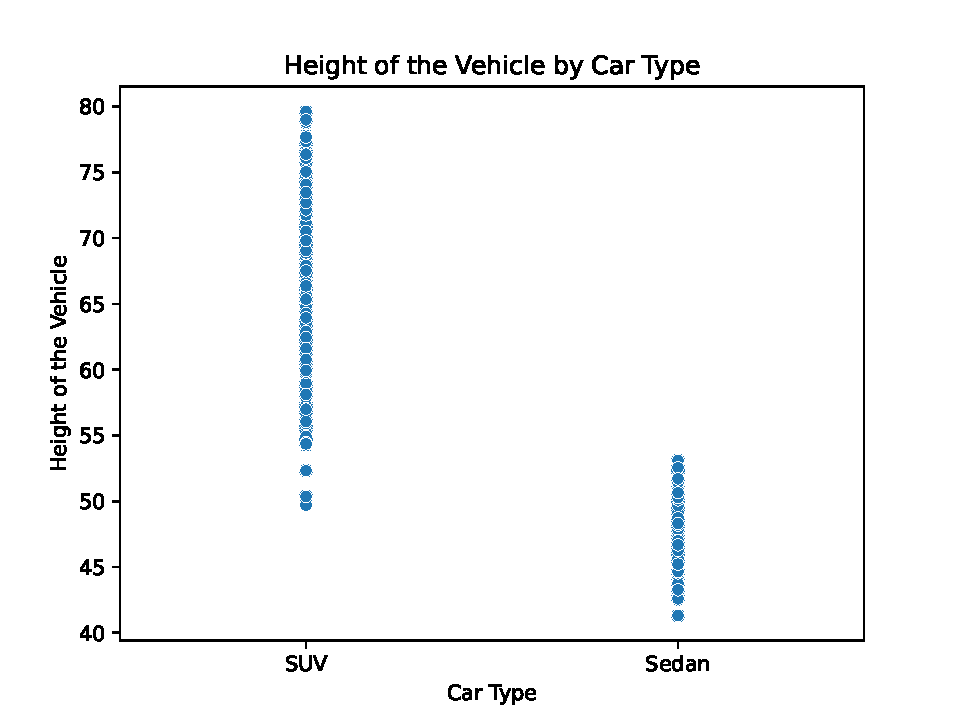
\includegraphics[width=0.4\textwidth]{./figure/exclusion_restriction_1.pdf}
    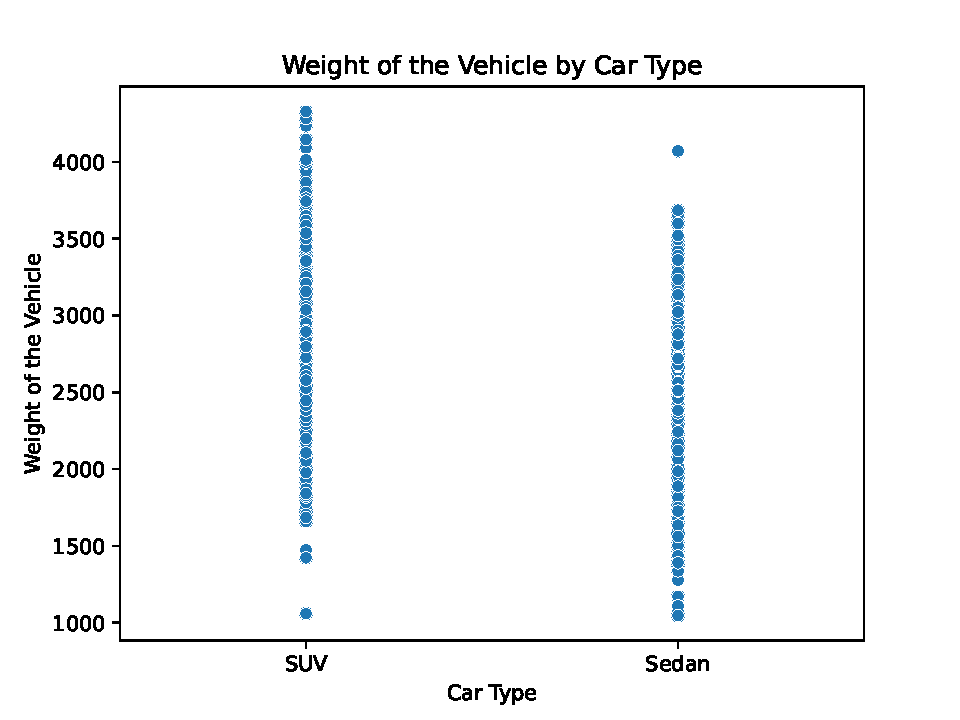
\includegraphics[width=0.4\textwidth]{./figure/exclusion_restriction_2.pdf}\\
    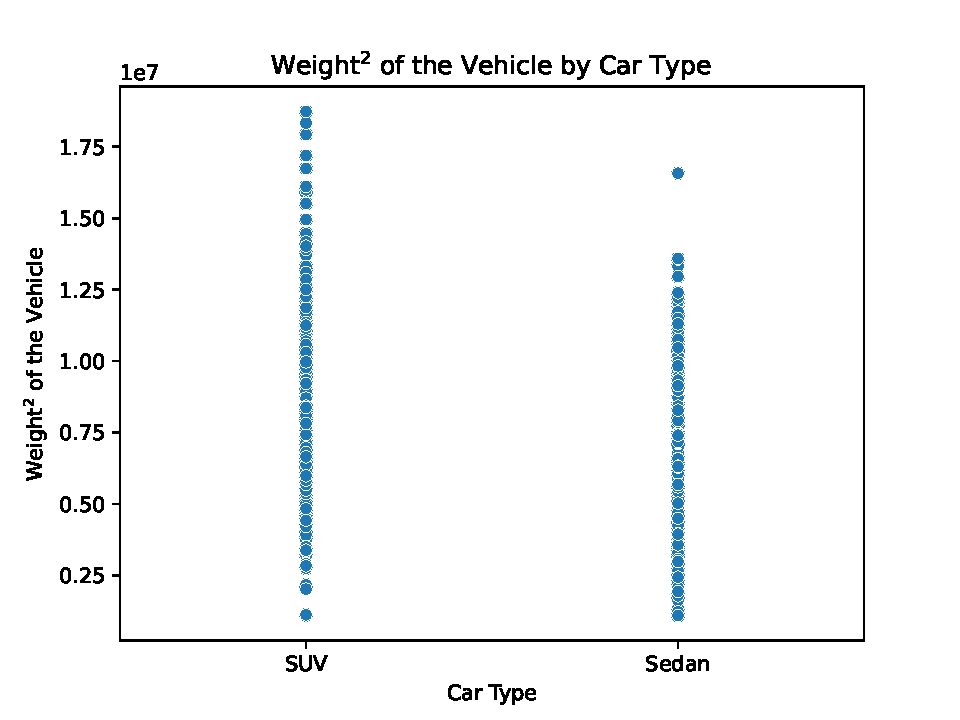
\includegraphics[width=0.4\textwidth]{./figure/exclusion_restriction_3.pdf}
    \caption{Scatter plot of variables used as IV and car type}
    \label{f1:exclusion} 
    \end{figure}
    

    \item[(e)] From the result in Table \ref{t1:2SLS}, the estimates from column (a) and (b) are statistically significant, and both are not statistically different. However, the estiamtes from column (c) is practically zero, with estimates that is very large.
\end{enumerate}
\item Table \ref{t2:2SLS_IVGMM} show the IVGMM estimates

\begin{table}[H]\centering
\caption{Comparing 2SLS and IVGMM estimates}
\label{t2:2SLS_IVGMM}
\begin{threeparttable}
\begin{tabular}{lcc}
\toprule
 & By Hand 2SLS & IVGMM \\
\midrule
Miles per gallon & 150.43 & 150.43 \\
  & (59.30) & (63.05) \\
=1 if the vehicle is sedan & -4676.09 & -4676.09 \\
  & (548.94) & (589.70) \\
\bottomrule
\end{tabular}

\end{threeparttable}
\end{table}

The discrepancy in the standard errors is because the standard error estimates in the by hand 2SLS is basically wrong if we use directly from the second stage estimates. To compute the correct standard errors, we need to compute the residuals correctly. The correct residuals is using the coefficient estimates from the second stage but using the original variables, i.e. $\hat{e_i}=X_i\hat{\beta}_{2^{nd} Stage}$. Instead what we use is the wrong residuals $\tilde{e_i}=\hat{X}_i\hat{\beta}_{2^{nd} Stage}$.
\end{enumerate}

\section*{Problem 2 Stata}
\begin{enumerate}
\item Table \ref{t3:IVLIML} shows the IV LIML estimates. The estimates are identical to the result from using IVGMM in the previous problem.
\begin{table}[H]\centering
\caption{IV LIML estimates}
\label{t3:IVLIML}
\begin{threeparttable}
\begin{tabular}{l*{2}{c}}
\hline\hline
                    &\multicolumn{1}{c}{Parameter Estimates}&\multicolumn{1}{c}{AME Estimates}\\
\hline
Constant            &      -0.769&            \\
                    &[-1.848,0.310]&            \\
=1 if home received retrofit&       0.904&    -110.729\\
                    &[0.893,0.916]&[-130.589,-90.869]\\
Square feet of home &       0.894&       0.622\\
                    &[0.880,0.909]&[0.607,0.638]\\
Outdoor average temperature (\textdegree F)&       0.281&       2.851\\
                    &[0.039,0.524]&[-2.057,7.758]\\
\hline
Observations        &       1,000&       1,000\\
\hline\hline
\end{tabular}

\end{threeparttable}
\end{table}
\item The effective F-stat and the critical value is 78.36 and 37.42, respectively. Based on \cite{pflueger2015robust} if the effective F-stat is greater than the critical value, then we can conclude that we rejects the null hypothesis that the instrument is weak.
\end{enumerate}
    
\bibliography{\bib}
\end{document}